\chapter{Theoretical Background}
\label{Chapter-Theoretical-Background}

%%%%%%%%%%%%%%%%%%%%%%%%%%%%%%%%%%%%%%%%%%%%%%%%%%%%%%%%%% Artificial Intelligence & Machine Learning %%%%%%%%%%%%%%%%%%%%%%%%%%%%%%%%%%%%%%%%%%%%%%%%%%%%%%%%%%
\section{Artificial Intelligence \& Machine Learning}

Various researchers and textbooks may provide different definitions of Artificial Intelligence (AI). Depending the school of though, AI is an artificial actor that thinks or acts, rationally or human-like, depending on what it knows. Generally, AI can be described as the study of intelligence agents. It is a modern science that encompasses a large variety of sub-fields, ranging from general-purpose areas, such as learning, to specific tasks like playing chess and giving medical diagnoses. AI can be relevant to any intellectual field, as it systematizes and automates intellectual tasks. \cite{russell_norvig_2003_1}

Machine learning (ML) is an AI field in which agents, in addition to the performance element, include a learning element that utilises their past experiences to enhance their behaviour. The core idea behind ML is that perception should be used to improve the ability to act in the future, not simply react in the present. Designing a learning element is a multi-facet problem that is affected by three major issues. \cite{russell_norvig_2003_18}

\subsection*{Information management}%TODO:find a better title
The first issue is determining what information what information is useful and how it should be utilized. Different components of the input and output data should be learnt depending on the context in which the learning actor operates. One method is to directly link the current state of the actor or the world to their actions. Sometimes it can be more appropriate to infer relevant patterns from the data while ignoring unnecessary information. Another way is to collect action-value information indicating the desirability of actions based on their effect in the world state. These and other options may need to be combined in order to extract the most meaningful knowledge from the available data.

Another key factor when designing learning systems is the availability of prior knowledge. Researchers have extensively looked into the issue where the agent uses only information that they encounter, but ways for transferring prior knowledge have been devised to speed up learning and improve decision-making.\cite{Transfer_Learning}

\subsection*{Feedback mechanism}
The type of feedback available has a significant impact on the design and is perhaps the most crucial aspect of the learning problem. Usually three major types are distinguished: supervised, unsupervised, and reinforcement learning.

Supervised learning problems involve learning functions between sets of inputs and outputs. This is the case of a fully observable environments where the effects of the actors actions are immediately visible or the existence of a third party providing the correct solutions.

Unsupervised learning problems, on the other hand, do not supply output values and learning patterns are solely based on the input. As it has no knowledge of what constitutes a correct action or a desired state, an unsupervised learning agent cannot learn what to do. This is a common scenario for probabilistic reasoning systems or when generating output data is prohibitively expensive. For the last case, a semi-supervised learning setting, in which only a subset of the outputs is generated, might be useful.

In the reinforcement learning setting there is no correct output provided, instead a reward is given to actor appropriate to the desirability of their actions. This is common when the world which the actor take part in continuously change according to their actions, or a desirable or undesirable state may be reached after a series of actions.

\subsection*{Representation of the learned information}
The representation of the learned information is another important factor in establishing how the learning algorithm should operate. Common schemes include linear weighted polynomials for utility functions, propositional or first order logic, probabilistic representations like Bayesian Networks\cite{Probabilistic_Reasoning} and ANNs\cite{McCulloch1943}, and other methods have all been created.

%%%%%%%%%%%%%%%%%%%%%%%%%%%%%%%%%%%%%%%%%%%%%%%%%%%%%%%%%%%%%%%%%%%%%%%% Deep learning %%%%%%%%%%%%%%%%%%%%%%%%%%%%%%%%%%%%%%%%%%%%%%%%%%%%%%%%%%%%%%%%%%%%%%%%%
\section{Deep learning}
Deep learning is a sub-field of ML, partially overlapping with big data science. It consists of algorithms that use the perceptron as their basic building block, which is a mathematical function based on the McCulloch-Pitts model of biological neurons. They typically have hundreds of thousands to millions of perceptors with a variety of designs and topologies. Deep learning architectures include Deep Neural Networks (DNN)s, Convolutional Neural Networks (CNN)s, Recurrent neural networks (RNN)s and others, each one offering different capabilities and options.

\begin{figure}[H]
    \centering
        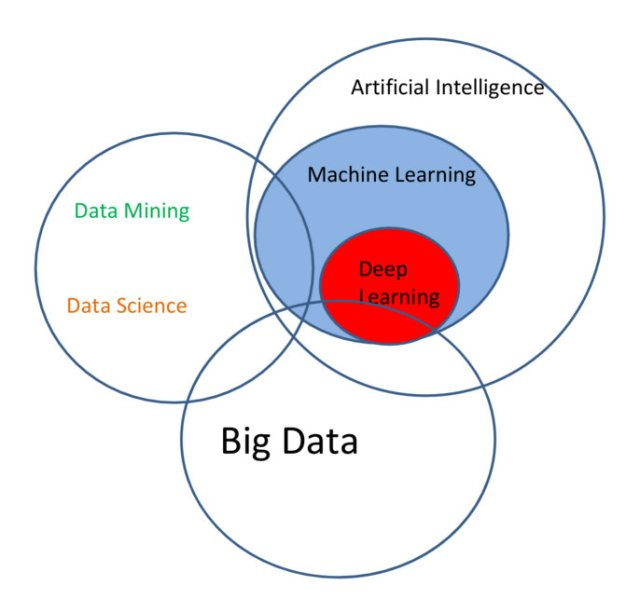
\includegraphics[scale=0.4]{Images/ai_data_science_diagram.jpg}
        \decoRule
        \caption[AI Venn Diagram]{AI, ML, DL, Data Mining, Data Science, and Big Data: \href{https://whatsthebigdata.com/2016/10/17/visually-linking-ai-machine-learning-deep-learning-big-data-and-data-science/}{URL}.}
        \label{fig:AI Venn Diagram}
\end{figure}

Deep learning applications have demonstrated human-like or superior capabilities in several scientific and commercial fields such as image\cite{Alexnet} and speech\cite{limits_speech_recognition} recognition, natural language processing\cite{natural_language}, climatology\cite{Climatology} and biotechnology\cite{biotechnology}. Due to these exceptional capabilities and wide range of applications, deep learning has attracted a large number of researchers from various scientific domains, resulting in its tremendous expansion. However, the science is still young and there are a number of challenges to be overcome. Expecting deep learning combined with improved data processing being a solution to computers gaining generic human-like intelligence (human equivalent AI) is still a distant dream.\cite{dl_evolution}

Historically, the field of deep learning emerged in 1943 with the inception of the aforementioned McCulloch-Pitts perceptron. In 1949, Donald Hebb noted out in his book "The Organization of Behavior" that neural pathways are strengthened each time they are utilized, a principle that is crucial to how humans learn. He claimed that when two nerves fire at the same moment, the link between them is strengthened. This progress resulted in the creation of the first real-world application of ANNs, "MADALINE" an adaptive filter that eliminates echoes on phone lines. In 1962, Widrow \& Hoff developed a learning procedure that distributed the error across the network, resulting in its eventual elimination. Despite these advances, deep learning research plummeted due to a variety of internal and external factor, including the widespread use of fundamentally faulty learning function and the adoption of von Neumann architecture across computer science.

Deep learning research stagnated until 1975, when developments such as Werbos' backpropagation and the building of the first multilayered network reignited interest in the field. Since then, the field continues to expand with innovations like hybrid models and ANN pooling layers. The current focus is on developing deep learning-specific hardware, as fast and efficient ANNs rely on it being defined for their use. Generally, architectures based on accelerators such as GPUs and FPGAs, or VLSI hardware-based designs, outperform CPU-based architectures. \cite{dl_history}


\subsection{Artificial Neuron \& activation function}

\begin{figure}[H]
    \centering
        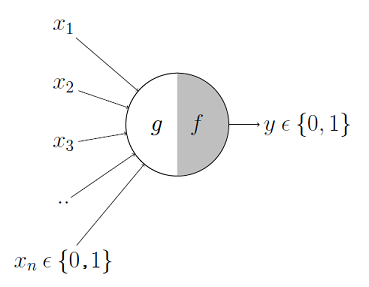
\includegraphics[scale=0.7]{Images/CNNArchitectures/McCulloch-Pitts Neuron.png}
        \decoRule
        \caption[McCulloch-Pitts Neuron]{The McCulloch-Pitts Neuron: \href{https://towardsdatascience.com/mcculloch-pitts-model-5fdf65ac5dd1}{URL}.}
        \label{fig:McCulloch-Pitts Neuron}
\end{figure}


\subsection{ANN architectures}
dnn
cnn
rnn
\subsection{Training Neural Networks}
\subsection{Model Overfitting}
FL smooths overfiting a bit, better talk about it. Maybe subsection of previous section?

%%%%%%%%%%%%%%%%%%%%%%%%%%%%%%%%%%%%%%%%%%%%%%%%%%%%%%%%%%%%%%%%%%%%%% Federated learning %%%%%%%%%%%%%%%%%%%%%%%%%%%%%%%%%%%%%%%%%%%%%%%%%%%%%%%%%%%%%%%%%%%%%%
\section{Federated Learning}
Lifecycle of a Model in Federated Learning / Typical Federated Training Process
\subsection{Data distribution}
iid - non iid
\subsection{Categorization}
horizontal - vertical - transfer learning?
\subsection{Architectures for a federated learning system}